\label{sec:model}
Our in-context function estimation model consist of an encoder and a decoder with two outputs. The encoder and the first decoder component can be interpreted as the Branch and Trunk nets from DeepONets \citet{Lu_2021}. Like \citet{seifner2025zeroshotimputationfoundationinference} we predict the mean and log variance of a gaussian distribution for each data point. \autoref{fig:model} shows our model architecture. We use the Attention is all you need transformer encoder from \citet{vaswani2017attention} with 10 layers to process the input sequence. The transformer encoder has a fixed number of channels and expects the input sequence to match in dimension. Including time indices and function values, our input sequence has two channels. The linear projection layer in the encoder projects the sequence to have the desired number of channels. Linear projections for a sequence with shared weights are equivalent to 1d-convolutions, like \citet{vaswani2017attention} we use 1d-convolutions for the linear projection in the encoder. The encoder outputs a sequence with the same length as the input sequence. To be processed by the feed forward networks of the decoder we need a fixed size vector as output. To fix the location of our desired output vector, we append a learnable token as the first element of the sequence. Therefore, we are ignoring all but the first element of the output sequence and this first element is forwarded to the decoder. This vector of fixed size is supposed to store all relevant information from the context points to predict all function values given the desired time index.

The decoder receives the hidden vector from the encoder, representing the input data and a single time index. This is the desired time to which the model is supposed to predict the function value. Like in the encoder the time index is projected to higher dimensions. Afterwards, it is concatenated with the hidden vector. This results in the number of decoder hidden dimension to be 50\% larger than the number of encoder hidden dimensions. In the decoder we are not dealing with sequences, so the linear projection is done by a feed forward network. The same is true for the feed forward layers within both decoder components. The two decoder components predict the mean and log variance for a specific point in time. When processing data during training and prediction, the input sequence of known context points is first processed by the encoder. Then the decoder is used to predict all points on a grid. We use a grid of 128 points on an interval of $[0,1]$. This means, we run the decoder 128 times with corresponding output time indices. The encoder result is only calculated once. 

\begin{figure}
		\centering
	\begin{tikzpicture}
	\node at (0,0) (A)  {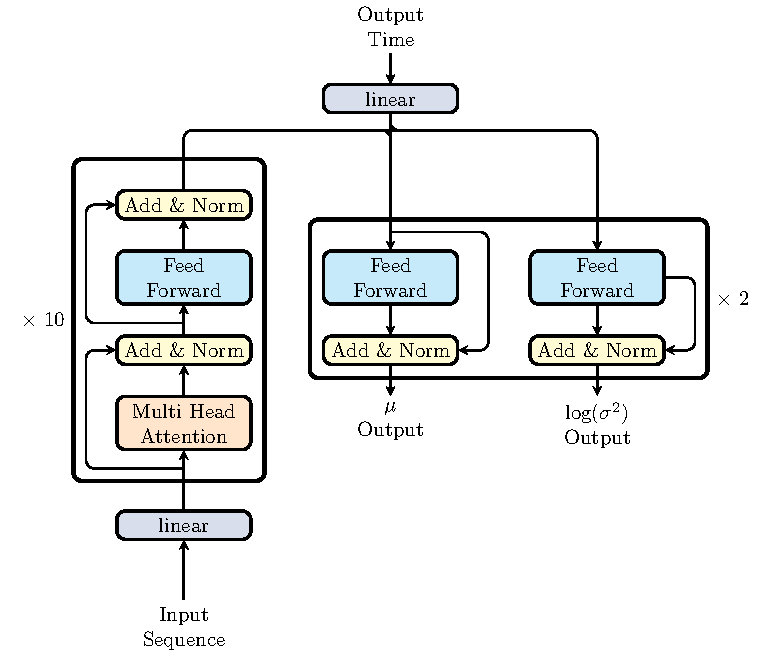
\includegraphics[width=\linewidth]{figures/architecture.pdf}};
	\end{tikzpicture}
	\caption{In-context function estimation model with an encoder on the left and two feed forward decoders on the right.}
	\label{fig:model}
\end{figure}

We normalize values and time indices as part of the model implementation. Like \citet{seifner2025zeroshotimputationfoundationinference} we employ min-max normalization for the input sequence (time indices and values). During training the target sequence is normalized as well and the loss is computed on the normalized data. This has the advantage, that all functions in one batch are weighed equally independent of the scale at which they are operating. \autoref{eq:norm} shows the general formula for normalizing data. During training, the min and max values for normalizing both input and target values are determined from the input data. When predicting results we denormalize the mean and standard deviation value. Denormalizing predicted mean values in \autoref{eq:denorm} differs from denormalizing the standard deviation in \autoref{eq:denorm_std}, as only its scale has to be denormalized. Note that \autoref{eq:denorm_std} includes the predicted log variance for completeness.

\begin{align}
x_i &\leftarrow \dfrac{x_i-x_{\text{min}}}{x_{\text{max}}-x_{\text{min}}} \label{eq:norm} \\
\mu &\leftarrow \mu (x_{\text{max}}-x_{\text{min}}) + x_{\text{min}} \label{eq:denorm} \\
\sigma &= \sqrt{e^{\text{log}(\sigma^2)}} x_{\text{max}}-x_{\text{min}} \label{eq:denorm_std} 
\end{align}



